% Options for packages loaded elsewhere
% Options for packages loaded elsewhere
\PassOptionsToPackage{unicode}{hyperref}
\PassOptionsToPackage{hyphens}{url}
\PassOptionsToPackage{dvipsnames,svgnames,x11names}{xcolor}
%
\documentclass[
  letterpaper,
  DIV=11,
  numbers=noendperiod]{scrartcl}
\usepackage{xcolor}
\usepackage{amsmath,amssymb}
\setcounter{secnumdepth}{-\maxdimen} % remove section numbering
\usepackage{iftex}
\ifPDFTeX
  \usepackage[T1]{fontenc}
  \usepackage[utf8]{inputenc}
  \usepackage{textcomp} % provide euro and other symbols
\else % if luatex or xetex
  \usepackage{unicode-math} % this also loads fontspec
  \defaultfontfeatures{Scale=MatchLowercase}
  \defaultfontfeatures[\rmfamily]{Ligatures=TeX,Scale=1}
\fi
\usepackage{lmodern}
\ifPDFTeX\else
  % xetex/luatex font selection
  \setmainfont[]{Georgia}
  \setsansfont[]{Avenir}
  \setmonofont[]{Menlo}
  \setmathfont[]{STIX Two Math}
\fi
% Use upquote if available, for straight quotes in verbatim environments
\IfFileExists{upquote.sty}{\usepackage{upquote}}{}
\IfFileExists{microtype.sty}{% use microtype if available
  \usepackage[]{microtype}
  \UseMicrotypeSet[protrusion]{basicmath} % disable protrusion for tt fonts
}{}
\makeatletter
\@ifundefined{KOMAClassName}{% if non-KOMA class
  \IfFileExists{parskip.sty}{%
    \usepackage{parskip}
  }{% else
    \setlength{\parindent}{0pt}
    \setlength{\parskip}{6pt plus 2pt minus 1pt}}
}{% if KOMA class
  \KOMAoptions{parskip=half}}
\makeatother
% Make \paragraph and \subparagraph free-standing
\makeatletter
\ifx\paragraph\undefined\else
  \let\oldparagraph\paragraph
  \renewcommand{\paragraph}{
    \@ifstar
      \xxxParagraphStar
      \xxxParagraphNoStar
  }
  \newcommand{\xxxParagraphStar}[1]{\oldparagraph*{#1}\mbox{}}
  \newcommand{\xxxParagraphNoStar}[1]{\oldparagraph{#1}\mbox{}}
\fi
\ifx\subparagraph\undefined\else
  \let\oldsubparagraph\subparagraph
  \renewcommand{\subparagraph}{
    \@ifstar
      \xxxSubParagraphStar
      \xxxSubParagraphNoStar
  }
  \newcommand{\xxxSubParagraphStar}[1]{\oldsubparagraph*{#1}\mbox{}}
  \newcommand{\xxxSubParagraphNoStar}[1]{\oldsubparagraph{#1}\mbox{}}
\fi
\makeatother

\usepackage{color}
\usepackage{fancyvrb}
\newcommand{\VerbBar}{|}
\newcommand{\VERB}{\Verb[commandchars=\\\{\}]}
\DefineVerbatimEnvironment{Highlighting}{Verbatim}{commandchars=\\\{\}}
% Add ',fontsize=\small' for more characters per line
\usepackage{framed}
\definecolor{shadecolor}{RGB}{241,243,245}
\newenvironment{Shaded}{\begin{snugshade}}{\end{snugshade}}
\newcommand{\AlertTok}[1]{\textcolor[rgb]{0.68,0.00,0.00}{#1}}
\newcommand{\AnnotationTok}[1]{\textcolor[rgb]{0.37,0.37,0.37}{#1}}
\newcommand{\AttributeTok}[1]{\textcolor[rgb]{0.40,0.45,0.13}{#1}}
\newcommand{\BaseNTok}[1]{\textcolor[rgb]{0.68,0.00,0.00}{#1}}
\newcommand{\BuiltInTok}[1]{\textcolor[rgb]{0.00,0.23,0.31}{#1}}
\newcommand{\CharTok}[1]{\textcolor[rgb]{0.13,0.47,0.30}{#1}}
\newcommand{\CommentTok}[1]{\textcolor[rgb]{0.37,0.37,0.37}{#1}}
\newcommand{\CommentVarTok}[1]{\textcolor[rgb]{0.37,0.37,0.37}{\textit{#1}}}
\newcommand{\ConstantTok}[1]{\textcolor[rgb]{0.56,0.35,0.01}{#1}}
\newcommand{\ControlFlowTok}[1]{\textcolor[rgb]{0.00,0.23,0.31}{\textbf{#1}}}
\newcommand{\DataTypeTok}[1]{\textcolor[rgb]{0.68,0.00,0.00}{#1}}
\newcommand{\DecValTok}[1]{\textcolor[rgb]{0.68,0.00,0.00}{#1}}
\newcommand{\DocumentationTok}[1]{\textcolor[rgb]{0.37,0.37,0.37}{\textit{#1}}}
\newcommand{\ErrorTok}[1]{\textcolor[rgb]{0.68,0.00,0.00}{#1}}
\newcommand{\ExtensionTok}[1]{\textcolor[rgb]{0.00,0.23,0.31}{#1}}
\newcommand{\FloatTok}[1]{\textcolor[rgb]{0.68,0.00,0.00}{#1}}
\newcommand{\FunctionTok}[1]{\textcolor[rgb]{0.28,0.35,0.67}{#1}}
\newcommand{\ImportTok}[1]{\textcolor[rgb]{0.00,0.46,0.62}{#1}}
\newcommand{\InformationTok}[1]{\textcolor[rgb]{0.37,0.37,0.37}{#1}}
\newcommand{\KeywordTok}[1]{\textcolor[rgb]{0.00,0.23,0.31}{\textbf{#1}}}
\newcommand{\NormalTok}[1]{\textcolor[rgb]{0.00,0.23,0.31}{#1}}
\newcommand{\OperatorTok}[1]{\textcolor[rgb]{0.37,0.37,0.37}{#1}}
\newcommand{\OtherTok}[1]{\textcolor[rgb]{0.00,0.23,0.31}{#1}}
\newcommand{\PreprocessorTok}[1]{\textcolor[rgb]{0.68,0.00,0.00}{#1}}
\newcommand{\RegionMarkerTok}[1]{\textcolor[rgb]{0.00,0.23,0.31}{#1}}
\newcommand{\SpecialCharTok}[1]{\textcolor[rgb]{0.37,0.37,0.37}{#1}}
\newcommand{\SpecialStringTok}[1]{\textcolor[rgb]{0.13,0.47,0.30}{#1}}
\newcommand{\StringTok}[1]{\textcolor[rgb]{0.13,0.47,0.30}{#1}}
\newcommand{\VariableTok}[1]{\textcolor[rgb]{0.07,0.07,0.07}{#1}}
\newcommand{\VerbatimStringTok}[1]{\textcolor[rgb]{0.13,0.47,0.30}{#1}}
\newcommand{\WarningTok}[1]{\textcolor[rgb]{0.37,0.37,0.37}{\textit{#1}}}

\usepackage{longtable,booktabs,array}
\usepackage{calc} % for calculating minipage widths
% Correct order of tables after \paragraph or \subparagraph
\usepackage{etoolbox}
\makeatletter
\patchcmd\longtable{\par}{\if@noskipsec\mbox{}\fi\par}{}{}
\makeatother
% Allow footnotes in longtable head/foot
\IfFileExists{footnotehyper.sty}{\usepackage{footnotehyper}}{\usepackage{footnote}}
\makesavenoteenv{longtable}
\usepackage{graphicx}
\makeatletter
\newsavebox\pandoc@box
\newcommand*\pandocbounded[1]{% scales image to fit in text height/width
  \sbox\pandoc@box{#1}%
  \Gscale@div\@tempa{\textheight}{\dimexpr\ht\pandoc@box+\dp\pandoc@box\relax}%
  \Gscale@div\@tempb{\linewidth}{\wd\pandoc@box}%
  \ifdim\@tempb\p@<\@tempa\p@\let\@tempa\@tempb\fi% select the smaller of both
  \ifdim\@tempa\p@<\p@\scalebox{\@tempa}{\usebox\pandoc@box}%
  \else\usebox{\pandoc@box}%
  \fi%
}
% Set default figure placement to htbp
\def\fps@figure{htbp}
\makeatother





\setlength{\emergencystretch}{3em} % prevent overfull lines

\providecommand{\tightlist}{%
  \setlength{\itemsep}{0pt}\setlength{\parskip}{0pt}}



 


\KOMAoption{captions}{tableheading}
\makeatletter
\@ifpackageloaded{caption}{}{\usepackage{caption}}
\AtBeginDocument{%
\ifdefined\contentsname
  \renewcommand*\contentsname{Table of contents}
\else
  \newcommand\contentsname{Table of contents}
\fi
\ifdefined\listfigurename
  \renewcommand*\listfigurename{List of Figures}
\else
  \newcommand\listfigurename{List of Figures}
\fi
\ifdefined\listtablename
  \renewcommand*\listtablename{List of Tables}
\else
  \newcommand\listtablename{List of Tables}
\fi
\ifdefined\figurename
  \renewcommand*\figurename{Figure}
\else
  \newcommand\figurename{Figure}
\fi
\ifdefined\tablename
  \renewcommand*\tablename{Table}
\else
  \newcommand\tablename{Table}
\fi
}
\@ifpackageloaded{float}{}{\usepackage{float}}
\floatstyle{ruled}
\@ifundefined{c@chapter}{\newfloat{codelisting}{h}{lop}}{\newfloat{codelisting}{h}{lop}[chapter]}
\floatname{codelisting}{Listing}
\newcommand*\listoflistings{\listof{codelisting}{List of Listings}}
\makeatother
\makeatletter
\makeatother
\makeatletter
\@ifpackageloaded{caption}{}{\usepackage{caption}}
\@ifpackageloaded{subcaption}{}{\usepackage{subcaption}}
\makeatother
\usepackage{bookmark}
\IfFileExists{xurl.sty}{\usepackage{xurl}}{} % add URL line breaks if available
\urlstyle{same}
\hypersetup{
  pdftitle={Assignment 02 Data Exploration},
  pdfauthor={Theresa Wohlever},
  colorlinks=true,
  linkcolor={blue},
  filecolor={Maroon},
  citecolor={Blue},
  urlcolor={Blue},
  pdfcreator={LaTeX via pandoc}}


\title{Assignment 02 Data Exploration}
\usepackage{etoolbox}
\makeatletter
\providecommand{\subtitle}[1]{% add subtitle to \maketitle
  \apptocmd{\@title}{\par {\large #1 \par}}{}{}
}
\makeatother
\subtitle{BQOM 2578 \textbar{} Data Mining}
\author{Theresa Wohlever}
\date{2025-09-17}
\begin{document}
\maketitle

\renewcommand*\contentsname{Table of contents}
{
\hypersetup{linkcolor=}
\setcounter{tocdepth}{2}
\tableofcontents
}

\section{Executive Summary}\label{executive-summary}

This dataset is from
\href{https://data.medicaid.gov/dataset/80956a7d-e343-54f3-94a7-45d41b34fc0b\#data-table}{Medicaid
Drug AMP Reporting}

The Data Cleaning and Preparation includes creating a Date column
generated from the corresponding year and Quarter columns and
categorizing drug types.

Of the drugs that can be categorized, the most commonly occurring are
those addressing hypertension and cardiac disease. This category is
heavily invested in by labeler companies, including 28 of the top 30
companies.

\section{Drug AMP Reporting -
Quarterly}\label{drug-amp-reporting---quarterly}

The dataset is from
\href{https://data.medicaid.gov/dataset/80956a7d-e343-54f3-94a7-45d41b34fc0b\#data-table}{Medicaid
Drug AMP Reporting} and described there:

\begin{quote}
\emph{Drugs that have been reported under the Medicaid Drug Rebate
Program along with an indication of whether or not the required Average
Manufacturer Price (AMP) was reported for each drug. All drugs are
identified in the file by the 11-digit National Drug Code, product name,
labeler name, and reported (R) or not reported (NR).}
\end{quote}

Raw data from Medicaid Drug AMP Reporting:
\url{https://data.medicaid.gov/dataset/80956a7d-e343-54f3-94a7-45d41b34fc0b\#data-table}

\begin{Shaded}
\begin{Highlighting}[]
\NormalTok{base\_FILENAME }\OtherTok{\textless{}{-}} \StringTok{"DrugAMPReportingQuarterly022025"} \DocumentationTok{\#\# tiny}

\NormalTok{csv\_FILE }\OtherTok{\textless{}{-}} \FunctionTok{paste}\NormalTok{(base\_FILENAME, }\StringTok{".csv"}\NormalTok{, }\AttributeTok{sep =} \StringTok{""}\NormalTok{)}
\NormalTok{csv\_OUT\_FILE }\OtherTok{\textless{}{-}} \FunctionTok{paste}\NormalTok{(base\_FILENAME, }\StringTok{"\_processed.csv"}\NormalTok{, }\AttributeTok{sep =} \StringTok{""}\NormalTok{) }

\NormalTok{raw\_amp\_df }\OtherTok{\textless{}{-}} \FunctionTok{read.csv}\NormalTok{(csv\_FILE, }\AttributeTok{stringsAsFactors =} \ConstantTok{FALSE}\NormalTok{) }
\end{Highlighting}
\end{Shaded}

\section{Data Discovery}\label{data-discovery}

Review Head, Tail, Dimensions, Column Headers, and Summary Statistics

\begin{verbatim}
                             Labeler.Name         NDC
1 FLUORITAB CORPORATION                   00288110601
2 FLUORITAB CORPORATION                   00288110602
3 FLUORITAB CORPORATION                   00288110610
4 FLUORITAB CORPORATION                   00288110699
5 FLUORITAB CORPORATION                   00288220101
6 FLUORITAB CORPORATION                   00288220102
                                                 FDA.Product.Name Status Year
1 SODIUM FLUORIDE I.I MG                                              NR 2013
2 SODIUM FLUORIDE 1.1 MG                                              NR 2013
3 SODIUM FLUORIDE 1.1MG                                               NR 2013
4 SODIUM FLUORIDE 1.1MG                                               NR 2013
5 SODIUM FLUORIDE 2.2MG                                               NR 2013
6 SODIUM FLUORIDE 2.2 MG                                              NR 2013
  Quarter
1       1
2       1
3       1
4       1
5       1
6       1
\end{verbatim}

\begin{verbatim}
                 Labeler.Name         NDC     FDA.Product.Name Status Year
2031672 BAUSCH HEALTH US, LLC 99207030060            ZIANA GEL      R 2025
2031673 BAUSCH HEALTH US, LLC 99207046630 SOLODYN 80MG TABLETS      R 2025
2031674 BAUSCH HEALTH US, LLC 99207052510      VANOS CREAM .1%      R 2025
2031675 BAUSCH HEALTH US, LLC 99207052530      VANOS CREAM .1%      R 2025
2031676 BAUSCH HEALTH US, LLC 99207052560      VANOS CREAM .1%      R 2025
2031677 BAUSCH HEALTH US, LLC 99207085060   LUZU Cream 1% 60gm      R 2025
        Quarter
2031672       2
2031673       2
2031674       2
2031675       2
2031676       2
2031677       2
\end{verbatim}

\begin{verbatim}
[1] 2031677       6
\end{verbatim}

\begin{verbatim}
[1] "Labeler.Name"     "NDC"              "FDA.Product.Name" "Status"          
[5] "Year"             "Quarter"         
\end{verbatim}

\begin{verbatim}
 Labeler.Name           NDC            FDA.Product.Name      Status         
 Length:2031677     Length:2031677     Length:2031677     Length:2031677    
 Class :character   Class :character   Class :character   Class :character  
 Mode  :character   Mode  :character   Mode  :character   Mode  :character  
                                                                            
                                                                            
                                                                            
      Year         Quarter     
 Min.   :2013   Min.   :1.000  
 1st Qu.:2016   1st Qu.:2.000  
 Median :2019   Median :2.000  
 Mean   :2019   Mean   :2.496  
 3rd Qu.:2022   3rd Qu.:3.000  
 Max.   :2025   Max.   :4.000  
\end{verbatim}

\section{Data Cleaning}\label{data-cleaning}

Random subset to improve analysis execution speed Cleans up labeler
company names by removing excessive spacing Cleans up Status

\begin{Shaded}
\begin{Highlighting}[]
\NormalTok{df }\OtherTok{\textless{}{-}}\NormalTok{raw\_amp\_df }\CommentTok{\# sample\_n(raw\_amp\_df, 10000)}
\FunctionTok{names}\NormalTok{(df)[}\FunctionTok{names}\NormalTok{(df) }\SpecialCharTok{==} \StringTok{"FDA.Product.Name"}\NormalTok{] }\OtherTok{\textless{}{-}} \StringTok{"Product"}


\DocumentationTok{\#\# Clean Up Status}
\NormalTok{df }\OtherTok{\textless{}{-}}\NormalTok{ df }\SpecialCharTok{\%\textgreater{}\%} \FunctionTok{mutate}\NormalTok{(}\AttributeTok{Status =} \FunctionTok{case\_when}\NormalTok{(}
    \FunctionTok{grepl}\NormalTok{(}\StringTok{"\^{}R}\SpecialCharTok{\textbackslash{}\textbackslash{}}\StringTok{s*$"}\NormalTok{, Status) }\SpecialCharTok{\textasciitilde{}} \StringTok{"R"}\NormalTok{,}
    \FunctionTok{grepl}\NormalTok{(}\StringTok{"NR"}\NormalTok{, Status) }\SpecialCharTok{\textasciitilde{}} \StringTok{"NR"}\NormalTok{,}
    \ConstantTok{TRUE} \SpecialCharTok{\textasciitilde{}} \ConstantTok{NA}
\NormalTok{  ))}


\CommentTok{\# Clean up labeler names (remove excessive spacing and formatting)}
\NormalTok{df}\SpecialCharTok{$}\NormalTok{Labeler\_Clean }\OtherTok{\textless{}{-}} \FunctionTok{str\_trim}\NormalTok{(}\FunctionTok{str\_replace\_all}\NormalTok{(df}\SpecialCharTok{$}\NormalTok{Labeler.Name, }\StringTok{"}\SpecialCharTok{\textbackslash{}\textbackslash{}}\StringTok{s+"}\NormalTok{, }\StringTok{" "}\NormalTok{))}
\end{Highlighting}
\end{Shaded}

\section{Data Preparation}\label{data-preparation}

\subsection{Date Column Creation}\label{date-column-creation}

\begin{itemize}
\tightlist
\item
  Combines Year and Quarter columns into a proper Date column for better
  temporal analysis
\item
  Converts quarters to actual dates (Q1 = January 1st, Q4 = October 1st)
\end{itemize}

\begin{Shaded}
\begin{Highlighting}[]
\CommentTok{\# Create a meaningful Date column by combining Year and Quarter}
\CommentTok{\# Convert quarter to actual dates for better temporal analysis}
\NormalTok{df}\SpecialCharTok{$}\NormalTok{Date }\OtherTok{\textless{}{-}} \FunctionTok{as.Date}\NormalTok{(}\FunctionTok{paste}\NormalTok{(df}\SpecialCharTok{$}\NormalTok{Year, (df}\SpecialCharTok{$}\NormalTok{Quarter }\SpecialCharTok{{-}} \DecValTok{1}\NormalTok{) }\SpecialCharTok{*} \DecValTok{3} \SpecialCharTok{+} \DecValTok{1}\NormalTok{, }\StringTok{"01"}\NormalTok{, }\AttributeTok{sep =} \StringTok{"{-}"}\NormalTok{))}
\end{Highlighting}
\end{Shaded}

\subsection{Drug Category
Classification}\label{drug-category-classification}

\begin{itemize}
\tightlist
\item
  Creates meaningful drug categories by analyzing FDA Product Names
\end{itemize}

\begin{Shaded}
\begin{Highlighting}[]
\DocumentationTok{\#\# Update with Dose}
\NormalTok{df }\OtherTok{\textless{}{-}}\NormalTok{ df }\SpecialCharTok{\%\textgreater{}\%}
  \FunctionTok{mutate}\NormalTok{(}\AttributeTok{dose =} \FunctionTok{str\_extract}\NormalTok{(Product, }\StringTok{"}\SpecialCharTok{\textbackslash{}\textbackslash{}}\StringTok{d+(?=}\SpecialCharTok{\textbackslash{}\textbackslash{}}\StringTok{s*MG)"}\NormalTok{))}


\DocumentationTok{\#\# Prep for Categories}
\NormalTok{products }\OtherTok{\textless{}{-}}\NormalTok{ df}\SpecialCharTok{$}\NormalTok{Product}
\NormalTok{escaped\_products }\OtherTok{\textless{}{-}} \FunctionTok{gsub}\NormalTok{(}\StringTok{"([][\{\}()+*\^{}$.|?}\SpecialCharTok{\textbackslash{}\textbackslash{}}\StringTok{])"}\NormalTok{, }\StringTok{"}\SpecialCharTok{\textbackslash{}\textbackslash{}\textbackslash{}\textbackslash{}\textbackslash{}\textbackslash{}}\StringTok{1"}\NormalTok{, }\FunctionTok{toupper}\NormalTok{(products))}
\NormalTok{product\_regex }\OtherTok{\textless{}{-}} \FunctionTok{paste}\NormalTok{(escaped\_products, }\AttributeTok{collapse =} \StringTok{"|"}\NormalTok{)}
\NormalTok{has\_products }\OtherTok{\textless{}{-}} \FunctionTok{nzchar}\NormalTok{(product\_regex) }\CommentTok{\# TRUE if pattern not empty}

\ControlFlowTok{if}\NormalTok{ (product\_regex }\SpecialCharTok{!=} \StringTok{""}\NormalTok{) \{}
\NormalTok{  df }\OtherTok{\textless{}{-}}\NormalTok{ df }\SpecialCharTok{\%\textgreater{}\%}
   \FunctionTok{mutate}\NormalTok{(}
      \AttributeTok{ProductUpper =} \FunctionTok{toupper}\NormalTok{(Product),}
      \AttributeTok{Drug\_Category =} \FunctionTok{case\_when}\NormalTok{(}
        \CommentTok{\# All products in the text file}
\NormalTok{        has\_products }\SpecialCharTok{\&}
  
        \CommentTok{\# Opioid/Combination Analgesic}
        \FunctionTok{str\_detect}\NormalTok{(ProductUpper, }\StringTok{"OXYCOD|HYDROCOD|MORPHIN|TRAMADOL|CODEINE|METHADONE|BUPRENORPHINE|FENTANYL|HYDROMORPHONE|PERCOCET|OXYCONTIN|NORCO|SUBOXONE|DURAMORPH|DEMEROL|DILAUDID|OPANA|ARYMO|ZOHYDRO|ROXICODONE|BELBUCA|BUNAVAIL|DOLOGESIC|METHADOSE"}\NormalTok{) }\SpecialCharTok{\textasciitilde{}} \StringTok{"Opioid/Combination Analgesic"}\NormalTok{,}
  
        \CommentTok{\# NSAIDs/Non{-}opioid Analgesic/Antipyretic}
        \FunctionTok{str\_detect}\NormalTok{(ProductUpper, }\StringTok{"IBUPROFEN|NAPROXEN|ACETAMINOPHEN|APAP|ASPIRIN|DICLOFENAC|KETOPROFEN|ETODOLAC|INDOMETHACIN|SALSALATE|OXAPROZIN|PIROXICAM|KETOROLAC|CELECOXIB|MELOXICAM|MEFENAMIC|FENOPROFEN|EXCEDRIN|GOODY|TYLENOL|PAIN RELIEF|CAPSAICIN|THERA{-}GESIC|MINERAL ICE|HEADACHE POWDER|ADVIL"}\NormalTok{) }\SpecialCharTok{\textasciitilde{}} \StringTok{"NSAIDs/Pain/Antipyretic"}\NormalTok{,}
  
        \CommentTok{\# Antidiabetic}
        \FunctionTok{str\_detect}\NormalTok{(ProductUpper, }\StringTok{"METFORMIN|GLIMEPIRIDE|GLIPIZIDE|GLYBURIDE|JANUMET|GLUCOVANCE|INVOKANA|JARDIANCE|TRESIBA|BASAGLAR|OZEMPIC|STEGLUJAN|SYNJARDY|TRULICITY|PIOLIGLITAZONE|JENTADUETO|BYDUREON|GLUCOPHAGE|ACTOS|AFREZZA|INSULIN|LANTUS|LEVEMIR"}\NormalTok{) }\SpecialCharTok{\textasciitilde{}} \StringTok{"Antidiabetic"}\NormalTok{,}
  
        \CommentTok{\# Statins/Cholesterol}
        \FunctionTok{str\_detect}\NormalTok{(ProductUpper, }\StringTok{"ATORVASTATIN|SIMVASTATIN|LOVASTATIN|PRAVASTATIN|FLUVASTATIN|ROSUVASTATIN|LIPITOR|EZETIMIBE|NIASPAN|FENOFIBRATE|FENOFIBRIC ACID|TRICOR|CRESTOR|VYTORIN|GEMFIBROZIL|FIBRICOR|LIPOPHEN|LOPID|OMEGA 3|EPA"}\NormalTok{) }\SpecialCharTok{\textasciitilde{}} \StringTok{"Lipid Modifier"}\NormalTok{,}
  
        \CommentTok{\# Antihypertensive/Cardiac}
        \FunctionTok{str\_detect}\NormalTok{(ProductUpper, }\StringTok{"LISINOPRIL|ENALAPRIL|LOSARTAN|VALSARTAN|QUINAPRIL|TELMISARTAN|OLMESARTAN|RAMIPRIL|BENAZEPRIL|CANDESARTAN|HCTZ|SPIRONOLACTONE|EPLE|TRIAMTERENE|BISOPROLOL|CARVEDILOL|LABETALOL|DILTIAZEM|FELDOPINE|VERAPAMIL|NIFEDIPINE|ISOSORBIDE|NITROGLYCERIN|RANOLAZINE|AMLODIPINE|PROPRANOLOL|BETAXOLOL|TAMSULOSIN|DOXAZOSIN|ALDACTAZIDE|POTASSIUM CHL|ATENOLOL|SOTALOL|METOPROLOL|CHLORTHALIDONE|HYDRALAZINE|CLONIDINE|GUANFACINE|METHYLDOPA|AMIODARONE|DIGOXIN|MILRINONE|SUCCINYLCHOLINE|MIDODRINE|MINOXIDIL|NEBIVOLOL|NADOLOL|PROROL|TERAZOSIN|DILTIAZ|VERELAN|INDAPAMIDE|BETAPACE|TRANDOLAPRIL|BYSTOLIC|MOEXIPRIL|FOSINOPRIL|CAPTOPRIL|ALISKIREN|MINIPRESS|PRAZOSIN"}\NormalTok{) }\SpecialCharTok{\textasciitilde{}} \StringTok{"Antihypertensive/Cardiac"}\NormalTok{,}
  
        \CommentTok{\# Diuretic/Electrolyte/Laxative/IV Fluid}
        \FunctionTok{str\_detect}\NormalTok{(ProductUpper, }\StringTok{"FUROSEMIDE|BUMETANIDE|HYDROCHLOROTHIAZIDE|HCTZ|CHLORTHALIDONE|METOLAZONE|TORSEMIDE|LACTULOSE|POLYETHYLENE GLYCOL|PEG|DOCUSATE|MINERAL OIL|BISACODYL|SENNA|CTL/MG|POTASSIUM|SODIUM|PHOSPHATE|BICARBONATE|MANITOL|MAGNESIUM|ELECTROLYTE|RENVELA|VIAFLEX|INFUVITE|PHOSPHA|CALCIUM ACETATE|PHOSPHATES|PLASMA{-}LYTE|PLASBUMIN"}\NormalTok{) }\SpecialCharTok{\textasciitilde{}} \StringTok{"Diuretic/Electrolyte/Laxative/IV"}\NormalTok{,}
  
        \CommentTok{\# Psychotropic/Antidepressant/Neuro}
        \FunctionTok{str\_detect}\NormalTok{(ProductUpper, }\StringTok{"SERTRALINE|FLUOXETINE|ESCITALOPRAM|CITALOPRAM|PAROXETINE|BUPROPION|VENLAFAXINE|DULOXETINE|AMITRIPTYLINE|NORTRIPTYLINE|IMIPRAMINE|DOXEPIN|MIRTAZAPINE|TRAZODONE|VORTIOXETINE|VILAZODONE|BUSPIRONE|DIAZEPAM|ALPRAZOLAM|LORAZEPAM|CLONAZEPAM|TEMAZEPAM|OXAZEPAM|ZOLPIDEM|ESZOPICLONE|ZOPICLONE|RAMELTEON|SUVOXAMELT|TRIAZOLAM|MELATONIN|DOTHIEPIN"}\NormalTok{) }\SpecialCharTok{\textasciitilde{}} \StringTok{"Psychotropic/Antidepressant/Neuro"}\NormalTok{,}
  
        \CommentTok{\# Antipsychotic/Neuroleptic}
        \FunctionTok{str\_detect}\NormalTok{(ProductUpper, }\StringTok{"QUETIAPINE|SEROQUEL|OLANZAPINE|ZYPREXA|RISPERIDONE|RISPERDAL|PALIPERIDONE|ARIPIPRAZOLE|ABILIFY|LURASIDONE|LATUDA|HALOPERIDOL|HALDOL|CHLORPROMAZINE|THIORIDAZINE|TRIFLUOPERAZINE|PERPHENAZINE|THIOTHIXENE|FLUPHENAZINE|CLOZAPINE|ASENAPINE|FANAPT|CARIPRAZINE|VRAYLAR|PIMOZIDE|MOLINDONE|ZELDOX|LOXAPINE"}\NormalTok{) }\SpecialCharTok{\textasciitilde{}} \StringTok{"Antipsychotic/Neuroleptic"}\NormalTok{,}
  
        \CommentTok{\# Anticonvulsant/Epilepsy/Neurologic}
        \FunctionTok{str\_detect}\NormalTok{(ProductUpper, }\StringTok{"LEVETIRACETAM|LAMOTRIGINE|TOPIRAMATE|DIVALPROEX|VALPROIC|GABAPENTIN|CARBAMAZEPINE|PREGABALIN|PHENYTOIN|PHENOBARBITAL|ZONISAMIDE|OXCARBAZEPINE|PRIMIDONE|BRIVARACETAM|LACOSAMIDE|TIAGABINE|ETHOSUXIMIDE|FELBAMATE|CLONAZEPAM|PERAMPANEL|VIGABATRIN|CENOBAMATE|LACOSAMIDE|GABRITRIL|FYCOMPA"}\NormalTok{) }\SpecialCharTok{\textasciitilde{}} \StringTok{"Anticonvulsant/Neurologic"}\NormalTok{,}
  
        \CommentTok{\# Antimicrobial/Antiinfective/Oncology/Immune}
        \FunctionTok{str\_detect}\NormalTok{(ProductUpper, }\StringTok{"AMOXICILLIN|CLAVULANATE|PENICILLIN|OXACILLIN|NAFCILLIN|AMPICILLIN|CEFAZOLIN|CEPHALEXIN|CEFTRIAXONE|CEFTAZIDIME|CEFTAROLINE|CEFEPIME|CEFUROXIME|CEFOTAXIME|CIPROFLOXACIN|LEVOFLOXACIN|MOXIFLOXACIN|OFLOXACIN|MINOCYCLINE|DOXYCYCLINE|ERYTHROMYCIN|AZITHROMYCIN|CLARITHROMYCIN|GENTAMICIN|TOBRAMYCIN|AMIKACIN|LINEZOLID|DAPTOMYCIN|VANCOMYCIN|RIFAMPIN|METRONIDAZOLE|TINIDAZOLE|CLINDAMYCIN|TRIMETHOPRIM|SULFAMETHOXAZOLE|TMP|NITROFURANTOIN|FOSFOMYCIN|MUPIROCIN|CLEOCIN|POLYMYXIN|COLISTIMETHATE|IMIPENEM|MEROPENEM|DORIPENEM|ERTAPENEM|AZTREONAM|CLOTRIMAZOLE|KETOCONAZOLE|FLUCONAZOLE|ITRACONAZOLE|POSACONAZOLE|VORICONAZOLE|CASPOFUNGIN|MICAFUNGIN|ANIDULAFUNGIN|NYSTATIN|AMPHOTERICIN|TERBINAFINE|GRISEOFULVIN|ACYCLOVIR|VALACYCLOVIR|FAMCICLOVIR|OSLTAMIVIR|BALOXAVIR|SOFOSBUVIR|LEDIPASVIR|RITONAVIR|LOPINAVIR|DARUNAVIR|ATAZANAVIR|INDINAVIR|SAQUINAVIR|DOLUTEGRAVIR|RALTEGRAVIR|ELVITEGRAVIR|BICTEGRAVIR|EMTRICITABINE|LAMIVUDINE|ABACAVIR|EFAVIRENZ|NEVIRAPINE|TENOFOVIR|ENTECAVIR|TELBIVUDINE|BOCEPREVIR|TELEPREVIR|GANCICLOVIR|VALGANCICLOVIR|CIDOFOVIR|FOSCARNET|LETROZOLE|TAMOXIFEN|FULVESTRANT|IMATINIB|ERLOTINIB|SORAFENIB|SUNITINIB|AFINITOR|EVEROLIMUS|NILUTAMIDE|POMALIDOMIDE|PEGINTERFERON|PLERIXAFOR|GEMCITABINE|CARBOPLATIN|DOXORUBICIN|CYCLOPHOSPHAMIDE|IFOSFAMIDE|BLEOMYCIN|MITOMYCIN|VINCRISTINE|VINBLASTINE|VINORELBINE|DAUNORUBICIN|CYTARABINE|TRETINOIN|THIOGUANINE|DOXEPIN|NIRAPARIB|INOTUZUMAB|BRENTUXIMAB|BLINATUMOMAB|IDELALISIB|OBINUTUZUMAB|RITUXIMAB|TRASTUZUMAB|PENICILLAMINE|AZATHIOPRINE|MYCOPHENOLATE|LEFLUNOMIDE|METHOTREXATE|FORTEO|DENOSUMAB|CINACALCET|CALCITRIOL|PTH|INSULIN DEGLUDEC"}\NormalTok{) }\SpecialCharTok{\textasciitilde{}} \StringTok{"Antimicrobial/Oncology/Immune"}\NormalTok{,}
  
        \CommentTok{\# Respiratory/ENT/Antihistamine}
        \FunctionTok{str\_detect}\NormalTok{(ProductUpper, }\StringTok{"ALBUTEROL|IPRATROPIUM|LEVOSALBUTAMOL|FORMOTEROL|BUDESONIDE|MONTELUKAST|SALMETEROL|FLUTICASONE|CROMOLYN|OLAPATADINE|AZELASTINE|ANTIHISTAMINE|LORATADINE|CETIRIZINE|FEXOFENADINE|DIPHENHYDRAMINE|PROMETHAZINE|PHENYLEPHRINE|PSEUDOEPHEDRINE|OXMETAZOLINE|RECTAL DECONGESTANT|COUGH|GUAIFENESIN|MUCINEX|DELSYM|RESPIRATORY|DM|EXPECTORANT|ANTITUSSIVE|CALDENSE|TUSSIN|NASAL|INHALE|INHALER|INH|INHALATION|NEBULIZER|DMX|NEBIVOLOL"}\NormalTok{) }\SpecialCharTok{\textasciitilde{}} \StringTok{"Respiratory/ENT/Antihistamine"}\NormalTok{,}
  
        \CommentTok{\# Hormonal/Endocrine}
        \FunctionTok{str\_detect}\NormalTok{(ProductUpper, }\StringTok{"LEVOTHYROXINE|LIOTHYRONINE|THYROID|ESTRADIOL|PROGESTERONE|MEDROXYPROGESTERONE|FINASTERIDE|FLUDROCORTISONE|HYDROCORTISONE|DEXAMETHASONE|METHYLPREDNISOLONE|PREDNISONE|SPIRONOLACTONE|TESTOSTERONE|VIVELLE|VIVELLE DOT|ACTEMRA|TAMOXIFEN|LETROZOLE|DROSPIRENONE|DRO+ETHIN+LEVO|MENEST|CONTRACEPTIVE|NORETHINDRONE|NORGESTIMATE|DESOGESTREL|LEVONORGESTREL|NEXPLANON|DEPO|PATCH"}\NormalTok{) }\SpecialCharTok{\textasciitilde{}} \StringTok{"Hormonal/Endocrine"}\NormalTok{,}
  
        \CommentTok{\# GI/GERD/Acid/IBD}
        \FunctionTok{str\_detect}\NormalTok{(ProductUpper, }\StringTok{"OMEPRAZOLE|PANTOPRAZOLE|LANSOPRAZOLE|ESOMEPRAZOLE|RABEPRAZOLE|FAMOTIDINE|RANITIDINE|CIMETIDINE|SUCRALFATE|PEPCID|BISMUTH|TUMS|ANTACID|CALCIUM CARBONATE|LAXATIVE|SENNA|BISACODYL|DOCUSATE|POLYETHYLENE GLYCOL|PEGLAX|BISMUTH SUBSALICYLATE|PEG|SODIUM BICARBONATE|REGULOID|FIBER|COLYTE|COLESTIPOL|CHOLESTYRAMINE|PREVALITE|COLCHICINE|LOPERAMIDE|IMODIUM|GAS RELIEF|SIMETHICONE|DICYCLOMINE|DIPHENOXYLATE|BILE SALT|STOOL SOFTENER|TAURINE|ASPIR{-}LOW|PRILOSEC|DUKORAL|BALSALAZIDE|MESALAMINE|SULFASALAZINE|ASACOL|UROSODIOL|URSODIOL|TYLONEX"}\NormalTok{) }\SpecialCharTok{\textasciitilde{}} \StringTok{"GI/IBD/GERD/Acid"}\NormalTok{,}
  
        \CommentTok{\# Anticoagulant/Platelet/Thrombolytic}
        \FunctionTok{str\_detect}\NormalTok{(ProductUpper, }\StringTok{"WARFARIN|COUMADIN|HEPARIN|ENOXAPARIN|MRXABAN|APIXABAN|XARELTO|PRADAXA|DABIGATRAN|FONDAPARINUX|LOVENOX|CLOPIDOGREL|PRASUGREL|TICAGRELOR|DIPYRIDAMOLE|PLAVIX|ALTEPLASE|ACTIVASE|THROMBOLYTIC|ARGATROBAN|BIVALIRUDIN|PROTAMINE|TPLASE|TISSEEL|THROMBIN|FACTOR IX|VII|VIII|RETROVIR|PROCRIT|EPOGEN|ERYTHROPOIETIN|RETACRIT"}\NormalTok{) }\SpecialCharTok{\textasciitilde{}} \StringTok{"Anticoagulant/Platelet/Thrombolytic"}\NormalTok{,}
  
        \CommentTok{\# Smoking Cessation}
        \FunctionTok{str\_detect}\NormalTok{(ProductUpper, }\StringTok{"NICOTINE|NICORETTE|NICODERM|NICOTROL|GUM|LOZENGE|PATCH|VARENICLINE|CHANTIX"}\NormalTok{) }\SpecialCharTok{\textasciitilde{}} \StringTok{"Smoking Cessation"}\NormalTok{,}
  
        \CommentTok{\# Reproductive/Contraceptive}
        \FunctionTok{str\_detect}\NormalTok{(ProductUpper, }\StringTok{"DROSPIRENONE|NORETHINDRONE|NORGESTIMATE|LEVONORGESTREL|ETHINYL ESTRADIOL|DESOGESTREL|ESTROSTEP|ORTHO|LOESTRIN|ORAL CONTRACEPTIVE|PATCH|NEXPLANON|VIVELLE|VIVELLE DOT|MENEST|ESTRACE|ESTROGEN|PROGESTIN|YAZ|YASMIN|MARVELON|MIRENA|PARAGARD|LO LOESTRIN|LUTERA|JULBER"}\NormalTok{) }\SpecialCharTok{\textasciitilde{}} \StringTok{"Contraceptive"}\NormalTok{,}
  
        \CommentTok{\# Vitamins/Nutrition}
        \FunctionTok{str\_detect}\NormalTok{(ProductUpper, }\StringTok{"VITAMIN|FOLIC|FOLATE|FOLIVANE|CITRANATAL|FERROUS|CYANOCOBALAMIN|NEONATAL COMPLETE|ERGOCALCIFEROL|AQUASOL|VITAFOL|MULTIVIT|PEDIATRIC|CHILDREN\textquotesingle{}S|CALCIFEROL|VITAMIN D"}\NormalTok{) }\SpecialCharTok{\textasciitilde{}} \StringTok{"Vitamins/Nutrition"}\NormalTok{,}
  
        \CommentTok{\# Dermatologic/Topical}
        \FunctionTok{str\_detect}\NormalTok{(ProductUpper, }\StringTok{"HYDROCORTISONE|CLOBETASOL|BETAMETHASONE|TRIAMCINOLONE|DESONIDE|DESOXIMETASONE|FLUOCINOLONE|ELIDEL|IMIQUIMOD|TRETINOIN|RETIN{-}A|BENZOYL PEROXIDE|MOISTURIZING|UREA CREAM|TRIAMCINOLONE|BACITRACIN|KETOCONAZOLE|CLOTRIMAZOLE|SILVER SULFADIAZINE|SELENIUM SULFIDE|TERBINAFINE|LINDANE|CICLOPIROX|A\&D OINTMENT|CALCIPOTRIENE|CALCITRENE|LUXIQ|MOISTURIZER|DAIVONEX|SUNSCREEN|LIDOFLEX|ANTIFUNGAL|SALICYLIC ACID|POLYSPORIN|TRIPLE ANTIBIOTIC|PRAMOXINE|CORTAID|ANUSOL|ALPHA KERI|ALCLOMETASONE"}\NormalTok{) }\SpecialCharTok{\textasciitilde{}} \StringTok{"Topical/Dermatologic"}\NormalTok{,}
  
        \CommentTok{\# Urologic/Bladder}
        \FunctionTok{str\_detect}\NormalTok{(ProductUpper, }\StringTok{"OXYBUTYNIN|TOLTERODINE|SOLIFENACIN|MIRABEGRON|TAMSULOSIN|FINASTERIDE|DUTASTERIDE|PHENAZOPYRIDINE|VESICARE|MYRBETRIQ|FESOTERODINE|DUTASTERIDE|TAMSULOSIN|UROGESIC|FESOTERODINE|TROSPIM|PRAZO"}\NormalTok{) }\SpecialCharTok{\textasciitilde{}} \StringTok{"Urologic/Bladder"}\NormalTok{,}
  
        \CommentTok{\# Miscellaneous/Other}
        \ConstantTok{TRUE} \SpecialCharTok{\textasciitilde{}} \StringTok{"Other"}
\NormalTok{      )}
\NormalTok{    ) }\SpecialCharTok{\%\textgreater{}\%}
    \FunctionTok{select}\NormalTok{(}\SpecialCharTok{{-}}\NormalTok{ProductUpper) }

\NormalTok{\} }\ControlFlowTok{else}\NormalTok{\{ }\FunctionTok{stop}\NormalTok{(}\StringTok{"Product Regex Empty!"}\NormalTok{) \}}

\NormalTok{Others }\OtherTok{\textless{}{-}}\NormalTok{ df }\SpecialCharTok{\%\textgreater{}\%} \FunctionTok{filter}\NormalTok{(Drug\_Category }\SpecialCharTok{==} \StringTok{"Other"}\NormalTok{) }\SpecialCharTok{\%\textgreater{}\%} \FunctionTok{distinct}\NormalTok{(Product) }\SpecialCharTok{\%\textgreater{}\%} \FunctionTok{pull}\NormalTok{(Product)}
\NormalTok{df\_noOther }\OtherTok{\textless{}{-}}\NormalTok{ df }\SpecialCharTok{\%\textgreater{}\%} \FunctionTok{filter}\NormalTok{(Drug\_Category }\SpecialCharTok{!=} \StringTok{"Other"}\NormalTok{)}
\end{Highlighting}
\end{Shaded}

\begin{Shaded}
\begin{Highlighting}[]
\CommentTok{\# Graph 2: Drug Categories by Registration Status}
\NormalTok{p2 }\OtherTok{\textless{}{-}} \FunctionTok{ggplot}\NormalTok{(df\_noOther, }\FunctionTok{aes}\NormalTok{(}\AttributeTok{x =} \FunctionTok{reorder}\NormalTok{(Drug\_Category, Drug\_Category, }\ControlFlowTok{function}\NormalTok{(x) }\FunctionTok{length}\NormalTok{(x)), }
                     \AttributeTok{fill =}\NormalTok{ Status)) }\SpecialCharTok{+}
  \FunctionTok{geom\_bar}\NormalTok{(}\AttributeTok{position =} \StringTok{"dodge"}\NormalTok{, }\AttributeTok{alpha =} \FloatTok{0.8}\NormalTok{) }\SpecialCharTok{+}
  \FunctionTok{coord\_flip}\NormalTok{() }\SpecialCharTok{+}
  \FunctionTok{labs}\NormalTok{(}\AttributeTok{title =} \StringTok{"Drug Categories by Registration Status"}\NormalTok{,}
       \AttributeTok{subtitle =} \StringTok{"Distribution of product categories and their registration status"}\NormalTok{,}
       \AttributeTok{x =} \StringTok{"Drug Category"}\NormalTok{,}
       \AttributeTok{y =} \StringTok{"Number of Products"}\NormalTok{,}
       \AttributeTok{fill =} \StringTok{"Status"}\NormalTok{,}
       \AttributeTok{caption =} \StringTok{"Categories derived from FDA Product Names"}\NormalTok{) }\SpecialCharTok{+}
  \FunctionTok{scale\_fill\_manual}\NormalTok{(}\AttributeTok{values =} \FunctionTok{c}\NormalTok{(}\StringTok{"NR"} \OtherTok{=} \StringTok{"\#E74C3C"}\NormalTok{, }\StringTok{"R"} \OtherTok{=} \StringTok{"\#27AE60"}\NormalTok{),}
                    \AttributeTok{labels =} \FunctionTok{c}\NormalTok{(}\StringTok{"NR"} \OtherTok{=} \StringTok{"Non{-}Registered"}\NormalTok{, }\StringTok{"R"} \OtherTok{=} \StringTok{"Registered"}\NormalTok{)) }\SpecialCharTok{+}
  \FunctionTok{theme\_minimal}\NormalTok{() }\SpecialCharTok{+}
  \FunctionTok{theme}\NormalTok{(}\AttributeTok{plot.title =} \FunctionTok{element\_text}\NormalTok{(}\AttributeTok{hjust =} \FloatTok{0.5}\NormalTok{, }\AttributeTok{size =} \DecValTok{14}\NormalTok{, }\AttributeTok{face =} \StringTok{"bold"}\NormalTok{),}
        \AttributeTok{plot.subtitle =} \FunctionTok{element\_text}\NormalTok{(}\AttributeTok{hjust =} \FloatTok{0.5}\NormalTok{, }\AttributeTok{size =} \DecValTok{12}\NormalTok{),}
        \AttributeTok{axis.text.y =} \FunctionTok{element\_text}\NormalTok{(}\AttributeTok{size =} \DecValTok{10}\NormalTok{))}

\FunctionTok{print}\NormalTok{(p2)}
\end{Highlighting}
\end{Shaded}

\pandocbounded{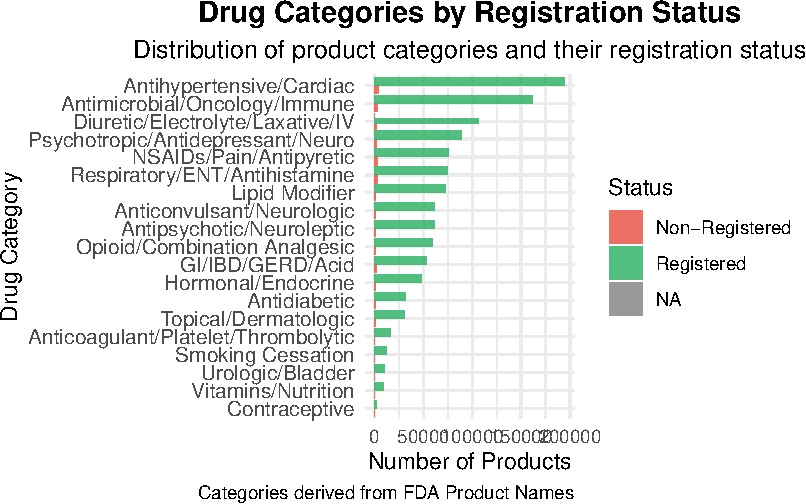
\includegraphics[keepaspectratio]{02-explore_files/figure-pdf/StatusCategoriesDistribution-1.pdf}}

\subsection{Category vs.~Labeler}\label{category-vs.-labeler}

\begin{Shaded}
\begin{Highlighting}[]
\CommentTok{\# Find top labelers by product count}
\NormalTok{top\_labelers }\OtherTok{\textless{}{-}}\NormalTok{ df }\SpecialCharTok{\%\textgreater{}\%}
  \FunctionTok{count}\NormalTok{(Labeler\_Clean, }\AttributeTok{sort =} \ConstantTok{TRUE}\NormalTok{) }\SpecialCharTok{\%\textgreater{}\%}
  \FunctionTok{slice\_head}\NormalTok{(}\AttributeTok{n =} \DecValTok{30}\NormalTok{) }\SpecialCharTok{\%\textgreater{}\%}
  \FunctionTok{pull}\NormalTok{(Labeler\_Clean)}

\CommentTok{\# Filter the main dataframe for these labelers}
\NormalTok{df\_top }\OtherTok{\textless{}{-}}\NormalTok{ df\_noOther }\SpecialCharTok{\%\textgreater{}\%}
  \FunctionTok{filter}\NormalTok{(Labeler\_Clean }\SpecialCharTok{\%in\%}\NormalTok{ top\_labelers)}

\CommentTok{\# 1. Summarize counts}
\NormalTok{df\_top\_counts }\OtherTok{\textless{}{-}}\NormalTok{ df\_top }\SpecialCharTok{\%\textgreater{}\%}
  \FunctionTok{count}\NormalTok{(Labeler\_Clean, Drug\_Category)  }

\CommentTok{\# 2. Plot heatmap}
\NormalTok{p\_heatmap }\OtherTok{\textless{}{-}} \FunctionTok{ggplot}\NormalTok{(df\_top\_counts, }\FunctionTok{aes}\NormalTok{(}\AttributeTok{x =}\NormalTok{ Drug\_Category, }\AttributeTok{y =}\NormalTok{ Labeler\_Clean, }\AttributeTok{fill =}\NormalTok{ n)) }\SpecialCharTok{+}
  \FunctionTok{geom\_tile}\NormalTok{(}\AttributeTok{color =} \StringTok{"white"}\NormalTok{) }\SpecialCharTok{+}
  \FunctionTok{scale\_fill\_gradient}\NormalTok{(}\AttributeTok{low =} \StringTok{"white"}\NormalTok{, }\AttributeTok{high =} \StringTok{"blue"}\NormalTok{) }\SpecialCharTok{+}
  \FunctionTok{theme\_minimal}\NormalTok{() }\SpecialCharTok{+}
  \FunctionTok{theme}\NormalTok{(}
    \AttributeTok{axis.text.x =} \FunctionTok{element\_text}\NormalTok{(}\AttributeTok{angle =} \DecValTok{90}\NormalTok{, }\AttributeTok{vjust =} \FloatTok{0.5}\NormalTok{, }\AttributeTok{hjust =} \DecValTok{1}\NormalTok{),}
    \AttributeTok{axis.text.y =} \FunctionTok{element\_text}\NormalTok{(}\AttributeTok{size =} \DecValTok{8}\NormalTok{) }\CommentTok{\# Decrease labeler font size}
\NormalTok{  ) }\SpecialCharTok{+}
  \FunctionTok{labs}\NormalTok{(}
    \AttributeTok{x =} \StringTok{"Category"}\NormalTok{,}
    \AttributeTok{y =} \StringTok{"Labeler"}\NormalTok{,}
    \AttributeTok{fill =} \StringTok{"Number of Products"}\NormalTok{,}
    \AttributeTok{title =} \StringTok{"Heatmap of Labeler vs Number of Products per Category"}
\NormalTok{  )}


\FunctionTok{print}\NormalTok{(p\_heatmap)}
\end{Highlighting}
\end{Shaded}

\pandocbounded{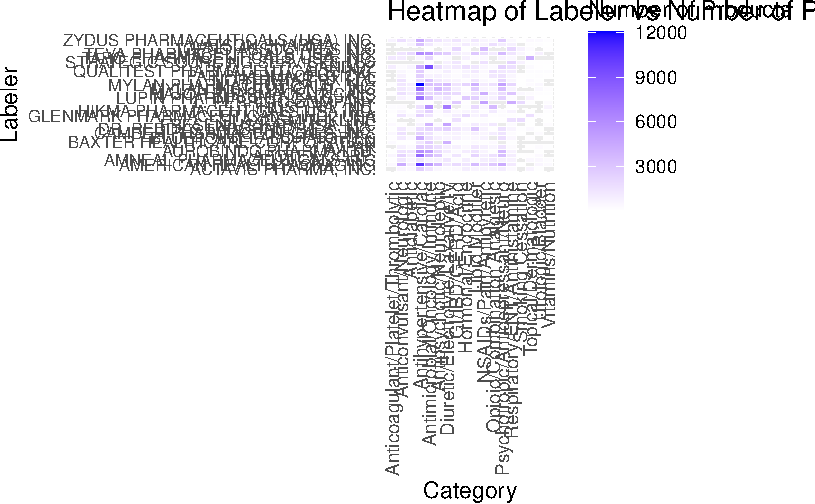
\includegraphics[keepaspectratio]{02-explore_files/figure-pdf/CategoryVsLabeler-1.pdf}}

\subsection{Distribution of Registration
Status}\label{distribution-of-registration-status}

\begin{Shaded}
\begin{Highlighting}[]
\NormalTok{p1 }\OtherTok{\textless{}{-}} \FunctionTok{ggplot}\NormalTok{(df, }\FunctionTok{aes}\NormalTok{(}\AttributeTok{x =}\NormalTok{ Status, }\AttributeTok{fill =}\NormalTok{ Status)) }\SpecialCharTok{+}
  \FunctionTok{geom\_bar}\NormalTok{(}\AttributeTok{stat =} \StringTok{"count"}\NormalTok{, }\AttributeTok{alpha =} \FloatTok{0.8}\NormalTok{) }\SpecialCharTok{+}
  \FunctionTok{geom\_text}\NormalTok{(}\AttributeTok{stat =} \StringTok{"count"}\NormalTok{, }\FunctionTok{aes}\NormalTok{(}\AttributeTok{label =} \FunctionTok{after\_stat}\NormalTok{(count)), }\AttributeTok{vjust =} \SpecialCharTok{{-}}\FloatTok{0.5}\NormalTok{) }\SpecialCharTok{+}
  \FunctionTok{labs}\NormalTok{(}\AttributeTok{title =} \StringTok{"Distribution of FDA Registration Status"}\NormalTok{,}
       \AttributeTok{subtitle =} \StringTok{"Comparison of Registered (R) vs Non{-}Registered (NR) Products"}\NormalTok{,}
       \AttributeTok{x =} \StringTok{"Registration Status"}\NormalTok{,}
       \AttributeTok{y =} \StringTok{"Number of Products"}\NormalTok{,}
       \AttributeTok{caption =} \StringTok{"Data Source: FDA Drug Registration Database"}\NormalTok{) }\SpecialCharTok{+}
  \FunctionTok{scale\_fill\_manual}\NormalTok{(}\AttributeTok{values =} \FunctionTok{c}\NormalTok{(}\StringTok{"NR"} \OtherTok{=} \StringTok{"\#E74C3C"}\NormalTok{, }\StringTok{"R"} \OtherTok{=} \StringTok{"\#27AE60"}\NormalTok{)) }\SpecialCharTok{+}
  \FunctionTok{theme\_minimal}\NormalTok{() }\SpecialCharTok{+}
  \FunctionTok{theme}\NormalTok{(}\AttributeTok{plot.title =} \FunctionTok{element\_text}\NormalTok{(}\AttributeTok{hjust =} \FloatTok{0.5}\NormalTok{, }\AttributeTok{size =} \DecValTok{14}\NormalTok{, }\AttributeTok{face =} \StringTok{"bold"}\NormalTok{),}
        \AttributeTok{plot.subtitle =} \FunctionTok{element\_text}\NormalTok{(}\AttributeTok{hjust =} \FloatTok{0.5}\NormalTok{, }\AttributeTok{size =} \DecValTok{12}\NormalTok{),}
        \AttributeTok{legend.position =} \StringTok{"none"}\NormalTok{)}

\FunctionTok{print}\NormalTok{(p1)}
\end{Highlighting}
\end{Shaded}

\pandocbounded{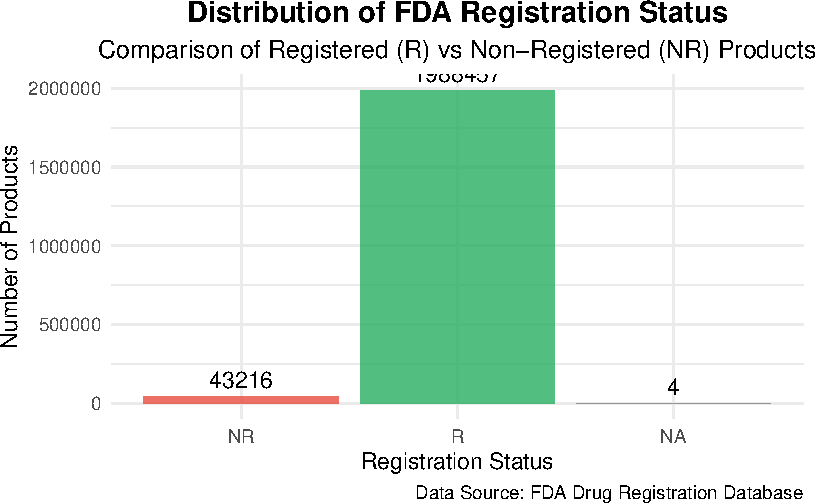
\includegraphics[keepaspectratio]{02-explore_files/figure-pdf/StatusDistribution-1.pdf}}

\begin{Shaded}
\begin{Highlighting}[]
\CommentTok{\# Graph 3: Top Pharmaceutical Companies (Top 30)}
\NormalTok{top\_labelers }\OtherTok{\textless{}{-}} \FunctionTok{names}\NormalTok{(}\FunctionTok{head}\NormalTok{(}\FunctionTok{sort}\NormalTok{(}\FunctionTok{table}\NormalTok{(df}\SpecialCharTok{$}\NormalTok{Labeler\_Clean), }\AttributeTok{decreasing =} \ConstantTok{TRUE}\NormalTok{), }\DecValTok{30}\NormalTok{))}
\NormalTok{df\_top }\OtherTok{\textless{}{-}}\NormalTok{ df[df}\SpecialCharTok{$}\NormalTok{Labeler\_Clean }\SpecialCharTok{\%in\%}\NormalTok{ top\_labelers, ]}

\NormalTok{p3 }\OtherTok{\textless{}{-}} \FunctionTok{ggplot}\NormalTok{(df\_top, }\FunctionTok{aes}\NormalTok{(}\AttributeTok{x =} \FunctionTok{reorder}\NormalTok{(Labeler\_Clean, Labeler\_Clean, }\ControlFlowTok{function}\NormalTok{(x) }\FunctionTok{length}\NormalTok{(x)),}
                         \AttributeTok{fill =}\NormalTok{ Status)) }\SpecialCharTok{+}
  \FunctionTok{geom\_bar}\NormalTok{(}\AttributeTok{stat =} \StringTok{"count"}\NormalTok{, }\AttributeTok{alpha =} \FloatTok{0.8}\NormalTok{) }\SpecialCharTok{+}
  \FunctionTok{coord\_flip}\NormalTok{() }\SpecialCharTok{+}
  \FunctionTok{labs}\NormalTok{(}\AttributeTok{title =} \StringTok{"Product Count by Top Pharmaceutical Companies"}\NormalTok{,}
       \AttributeTok{subtitle =} \StringTok{"Leading companies by number of products in the database"}\NormalTok{,}
       \AttributeTok{x =} \StringTok{"Pharmaceutical Company"}\NormalTok{,}
       \AttributeTok{y =} \StringTok{"Number of Products"}\NormalTok{,}
       \AttributeTok{fill =} \StringTok{"Registration Status"}\NormalTok{,}
       \AttributeTok{caption =} \StringTok{"Top Companies by product count"}\NormalTok{) }\SpecialCharTok{+}
  \FunctionTok{scale\_fill\_manual}\NormalTok{(}\AttributeTok{values =} \FunctionTok{c}\NormalTok{(}\StringTok{"NR"} \OtherTok{=} \StringTok{"\#E74C3C"}\NormalTok{, }\StringTok{"R"} \OtherTok{=} \StringTok{"\#27AE60"}\NormalTok{),}
                    \AttributeTok{labels =} \FunctionTok{c}\NormalTok{(}\StringTok{"NR"} \OtherTok{=} \StringTok{"Non{-}Registered"}\NormalTok{, }\StringTok{"R"} \OtherTok{=} \StringTok{"Registered"}\NormalTok{)) }\SpecialCharTok{+}
  \FunctionTok{theme\_minimal}\NormalTok{() }\SpecialCharTok{+}
  \FunctionTok{theme}\NormalTok{(}\AttributeTok{plot.title =} \FunctionTok{element\_text}\NormalTok{(}\AttributeTok{hjust =} \FloatTok{0.5}\NormalTok{, }\AttributeTok{size =} \DecValTok{14}\NormalTok{, }\AttributeTok{face =} \StringTok{"bold"}\NormalTok{),}
        \AttributeTok{plot.subtitle =} \FunctionTok{element\_text}\NormalTok{(}\AttributeTok{hjust =} \FloatTok{0.5}\NormalTok{, }\AttributeTok{size =} \DecValTok{12}\NormalTok{),}
        \AttributeTok{axis.text.y =} \FunctionTok{element\_text}\NormalTok{(}\AttributeTok{size =} \DecValTok{9}\NormalTok{))}

\FunctionTok{print}\NormalTok{(p3)}
\end{Highlighting}
\end{Shaded}

\pandocbounded{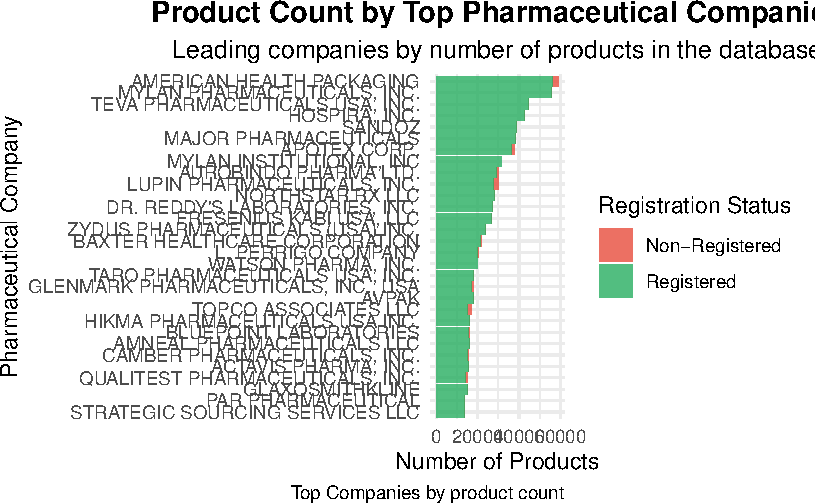
\includegraphics[keepaspectratio]{02-explore_files/figure-pdf/PharmaCompaniesDistribution-1.pdf}}

\begin{Shaded}
\begin{Highlighting}[]
\NormalTok{quarterly\_summary\_yearly }\OtherTok{\textless{}{-}}\NormalTok{ df }\SpecialCharTok{\%\textgreater{}\%}
  \FunctionTok{group\_by}\NormalTok{(Year, Status) }\SpecialCharTok{\%\textgreater{}\%}
  \FunctionTok{summarise}\NormalTok{(}\AttributeTok{count =} \FunctionTok{n}\NormalTok{(), }\AttributeTok{.groups =} \StringTok{\textquotesingle{}drop\textquotesingle{}}\NormalTok{)}

\NormalTok{p4 }\OtherTok{\textless{}{-}} \FunctionTok{ggplot}\NormalTok{(quarterly\_summary\_yearly, }\FunctionTok{aes}\NormalTok{(}\AttributeTok{x =} \FunctionTok{factor}\NormalTok{(Year), }\AttributeTok{y =}\NormalTok{ count, }\AttributeTok{fill =}\NormalTok{ Status)) }\SpecialCharTok{+}
  \FunctionTok{geom\_col}\NormalTok{(}\AttributeTok{position =} \StringTok{"stack"}\NormalTok{, }\AttributeTok{alpha =} \FloatTok{0.8}\NormalTok{, }\AttributeTok{width =} \FloatTok{0.7}\NormalTok{) }\SpecialCharTok{+}
  \FunctionTok{geom\_text}\NormalTok{(}\FunctionTok{aes}\NormalTok{(}\AttributeTok{label =}\NormalTok{ count), }\AttributeTok{position =} \FunctionTok{position\_stack}\NormalTok{(}\AttributeTok{vjust =} \FloatTok{0.5}\NormalTok{), }
            \AttributeTok{color =} \StringTok{"white"}\NormalTok{, }\AttributeTok{size =} \DecValTok{4}\NormalTok{, }\AttributeTok{fontface =} \StringTok{"bold"}\NormalTok{) }\SpecialCharTok{+}
  \FunctionTok{labs}\NormalTok{(}\AttributeTok{title =} \StringTok{"Pharmaceutical Product Registration Timeline"}\NormalTok{,}
       \AttributeTok{subtitle =} \StringTok{"Yearly distribution of registered vs non{-}registered products"}\NormalTok{,}
       \AttributeTok{x =} \StringTok{"Year"}\NormalTok{,}
       \AttributeTok{y =} \StringTok{"Number of Products"}\NormalTok{,}
       \AttributeTok{fill =} \StringTok{"Registration Status"}\NormalTok{,}
       \AttributeTok{caption =} \StringTok{""}\NormalTok{) }\SpecialCharTok{+}
  \FunctionTok{scale\_fill\_manual}\NormalTok{(}\AttributeTok{values =} \FunctionTok{c}\NormalTok{(}\StringTok{"NR"} \OtherTok{=} \StringTok{"\#E74C3C"}\NormalTok{, }\StringTok{"R"} \OtherTok{=} \StringTok{"\#27AE60"}\NormalTok{),}
                    \AttributeTok{labels =} \FunctionTok{c}\NormalTok{(}\StringTok{"NR"} \OtherTok{=} \StringTok{"Non{-}Registered"}\NormalTok{, }\StringTok{"R"} \OtherTok{=} \StringTok{"Registered"}\NormalTok{)) }\SpecialCharTok{+}
  \FunctionTok{theme\_minimal}\NormalTok{() }\SpecialCharTok{+}
  \FunctionTok{theme}\NormalTok{(}\AttributeTok{plot.title =} \FunctionTok{element\_text}\NormalTok{(}\AttributeTok{hjust =} \FloatTok{0.5}\NormalTok{, }\AttributeTok{size =} \DecValTok{14}\NormalTok{, }\AttributeTok{face =} \StringTok{"bold"}\NormalTok{),}
        \AttributeTok{plot.subtitle =} \FunctionTok{element\_text}\NormalTok{(}\AttributeTok{hjust =} \FloatTok{0.5}\NormalTok{, }\AttributeTok{size =} \DecValTok{12}\NormalTok{),}
        \AttributeTok{axis.text.x =} \FunctionTok{element\_text}\NormalTok{(}\AttributeTok{angle =} \DecValTok{0}\NormalTok{, }\AttributeTok{hjust =} \FloatTok{0.5}\NormalTok{))}

\FunctionTok{print}\NormalTok{(p4)}
\end{Highlighting}
\end{Shaded}

\pandocbounded{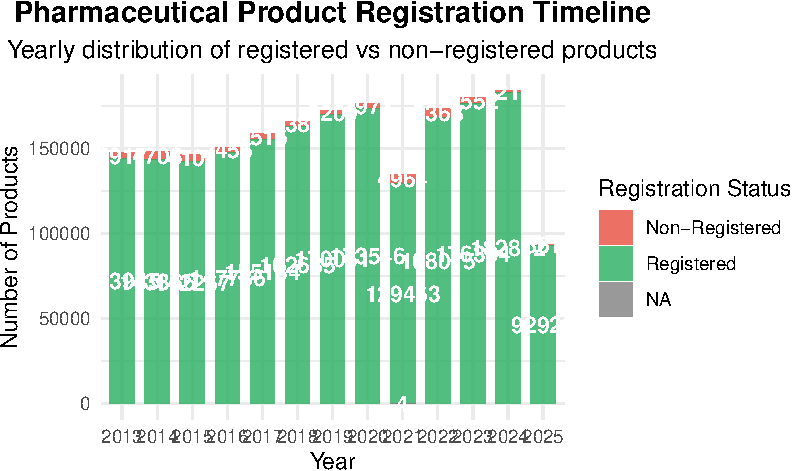
\includegraphics[keepaspectratio]{02-explore_files/figure-pdf/RegistrationTimelineDistribution-1.pdf}}

\section{Publishing}\label{publishing}

\begin{Shaded}
\begin{Highlighting}[]
\NormalTok{df}\SpecialCharTok{\%\textgreater{}\%}\FunctionTok{write.csv}\NormalTok{(csv\_OUT\_FILE,}\AttributeTok{row.names =} \ConstantTok{FALSE}\NormalTok{)}
\end{Highlighting}
\end{Shaded}





\end{document}
